\subsection{Skyroads}
Bei dem Spiel \textit{Skyroads} von \textit{Bluemoon} ist eine Art Jump and Run Spiel aus dem Jahr 1993. Ziel des Spiels ist es ein Raumschiff durch einen Parcour zu manövrieren. Der Spieler muss hierbei über Hindernisse oder Abgründe springen, beziehungsweise diesen ausweichen. Schafft er das Level nicht, kann er es beliebig oft neu starten. Das Prinzip des Spiels stammt aus dem Spiel \textit{Kosmonauts}, welches von den gleichen Entwicklern bereits im Jahre 1989 veröffentlicht wurde. Zu Beginn des Spiels stehen dem Nutzer bereits alle Levels zur Verfügung. Er kann in einer Übersichtsseite das gewünschte Level auswählen. \\
Mit \textit{Skyroads XMAS-Special} wurde 1994 ein Nachfolger veröffentlicht. Außerdem existieren mittlerweile sehr viele andere Spiele, die nach einer ähnlichen Spielmechanik funktionieren.
\begin{figure}[ht]
	\centering
	\begin{subfigure}{.45\textwidth}
	\centering
			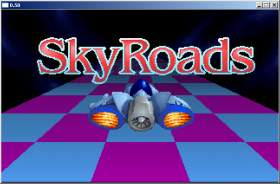
\includegraphics[width=.9\textwidth]{gfx/recherche/skyroads1.jpg}
	\end{subfigure}
	\begin{subfigure}{.45\textwidth}
	\centering
			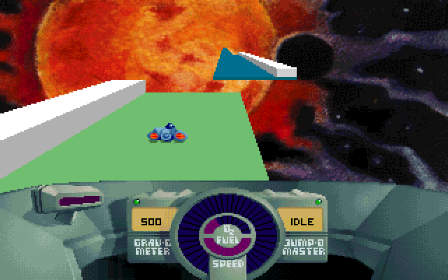
\includegraphics[width=.9\textwidth]{gfx/recherche/skyroads2.jpg}  
	\end{subfigure}
	\caption{Skyroads}
\end{figure}\\

\subsection{Audiosurf}

Das Geschicklichkeitsspiel \textit{Audiosurf} des Entwicklers \textit{Invisible Handlebar} aus dem Jahr 2008 ist ebenfalls ein Beispiel für eine vergleichbare Spielidee. Auch hier steuert der Spieler ein raumschiffartiges Gefährt über Bahnen und muss dabei Hindernissen ausweichen. Die Besonderheit dieses Spiels ist jedoch, wie der Name andeutet, dass die Strecken automatisch passend zu einem Musikstück generiert werden, das während des Spiels passend dazu abgespielt wird.\\
Je nach Spielmodus muss der Spieler farbige Blöcke auf den Bahnen einsammeln oder grauen Blöcken ausweichen. Die Blöcke werden dann als Rechtecke in einem Raster am unteren Bildschirmrand angesammelt, jeweils auf der Bahn, auf der sie eingesammelt wurden. Sobald drei oder mehr Blöcke gleicher Farbe aneinander angrenzen, blinken diese für wenige Sekunden und lösen sich dann auf, wobei der Spieler dafür Punkte erhält.\\
Ziel des Spiels ist es, auf diese Weise auf jeder Strecke bzw. jedem Lied möglichst viele Punkte zu sammeln. Diese Punkte werden dann auch in einer lokalen und globalen Highscore-Liste eingetragen. Eine weitere Motivation bieten verschiedene Bonusregelungen und Herausforderungen, wie beispielsweise. das Abschließen einer Strecke ohne dass sich am Ende noch Blöcke im Raster befinden oder die Strecke zu beenden ohne einen einzigen grauen Block berührt zu haben.\\
\begin{figure}[ht]
\centering
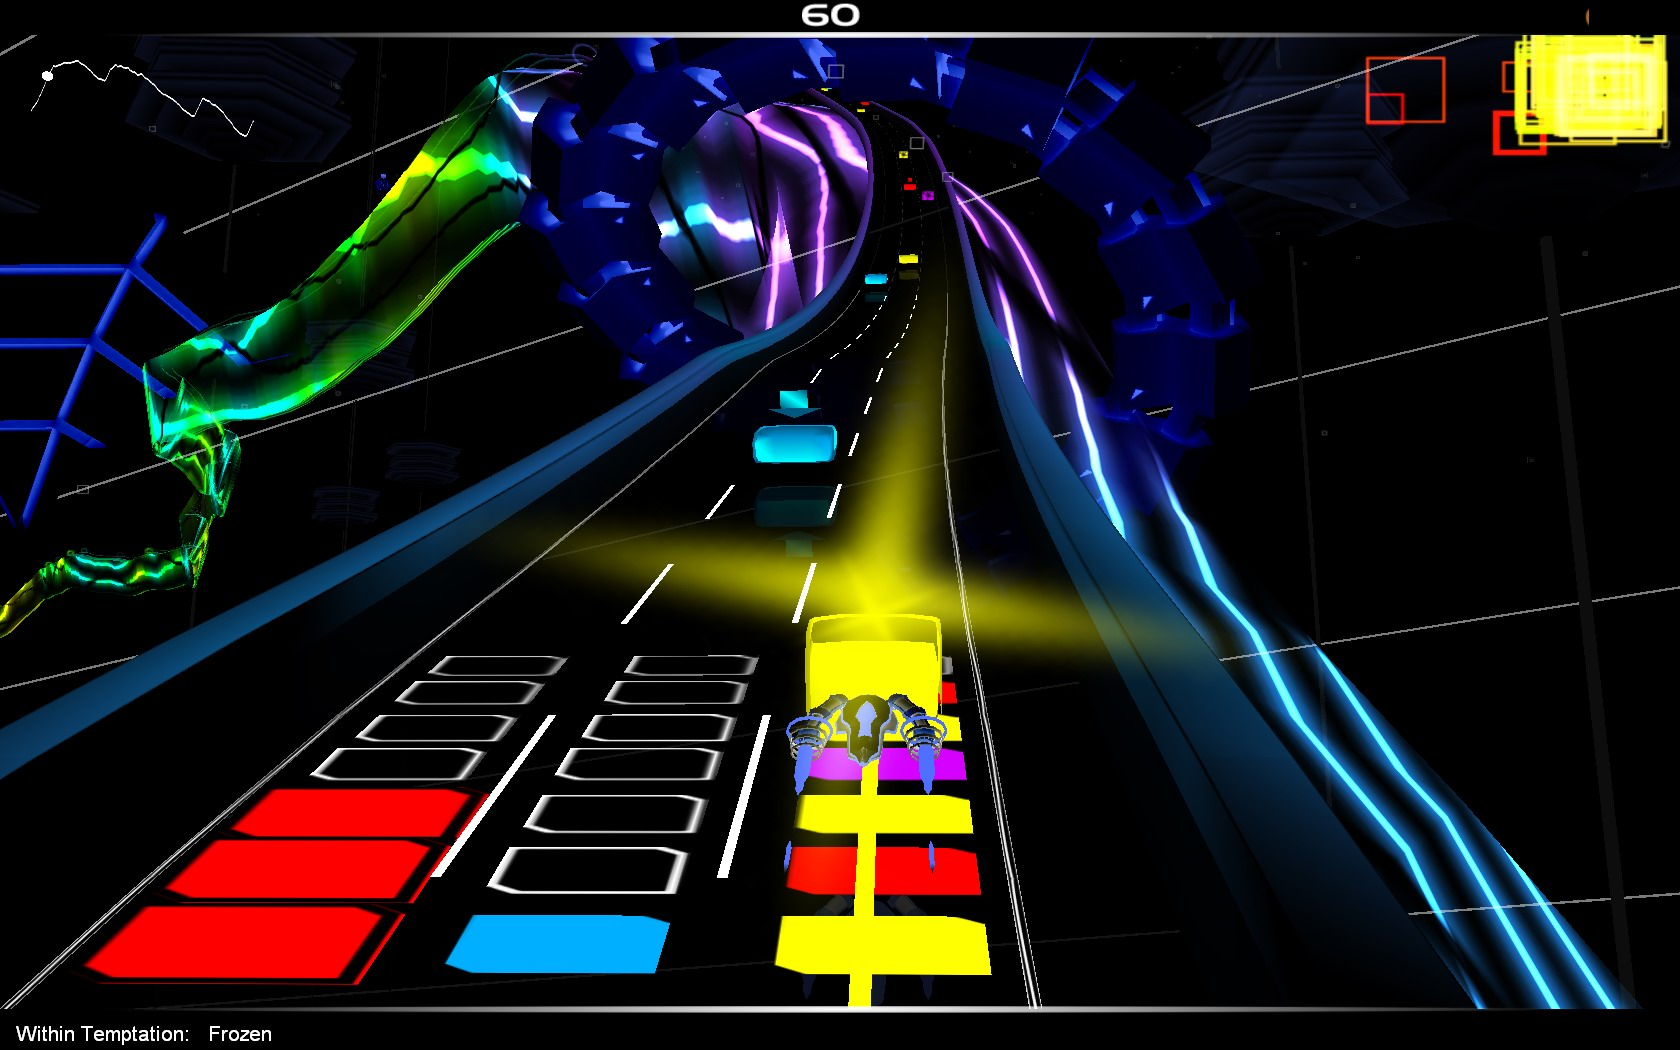
\includegraphics[width=.7\textwidth]{gfx/recherche/audiosurf.jpg}
\caption{Screenshot einer typischen Szene in Audiosurf\footnotemark}
\end{figure}
\footnotetext{Quelle: \url{https://market.myo.com/app/5474d1c6e4b081c4011c77b4/audiosurf-connector}}Ähnlich wie bei unserem Spiel handelt es sich also bei \textit{Audiosurf} um ein Geschicklichkeitsspiel, bei dem man ein Gefährt auf Bahnen hin- und herbewegt um Hindernissen auszuweichen. Anders ist jedoch vor allem, dass es bei \textit{Audiosurf} nicht darum geht, ein Level überhaupt zu schaffen, sondern die Motivation für den Spieler über ein Punkte- und Highscore-System generiert wird. Das wird auch dadurch deutlich, dass es in \textit{Audiosurf} nicht möglich ist, ein Level gar nicht zu schaffen. Kollisionen mit Hindernissen oder ein Überlaufen des Rasters führen hingegen nur zu einem Punktabzug, stören aber sonst nicht den Spielablauf.
